\chapter{Advanced UAV Control}
\section{Motivation}
\begin{figure}[thpb]
	\centering
	\framebox{\includegraphics[width=0.6\textwidth]{images/advanced_control_motivation.pdf}}
	\caption{Non-flat-earth model example. The unit optical axis vector $\hat{m}$ and the unit line of sight vector $\hat{l}$ are key components of the controller presented in this chapter.}
	\label{nonflatearth}
\end{figure}
The UAV control algorithm introduced in the previous chapter is relatively simple and easy to implement. Anyone with sound understanding of projective camera geometry and frame transformation would not have difficult time to implement the algorithm. However, the controller makes strong assumption that can be unrealistic for some cases. It assumes that the line of sight (LOS) vector to the target and the optical axis lie on the same flat surface which is often called 'flat-earth assumption'. Then, the altitude of multirotor acts as scale factor that had been lost due to the projective camera model to compute how much the UAV has to move forward. An advanced UAV controller presented in this chapter overcomes the flat-earth assumption by working out with the unit LOS vector and unit optical axis vector (see Figure \ref{nonflatearth}). Also, the controller does not require the altitude of multirotor to be known because the scale factor does not have to be recovered.

\section{Controller Derivation for Simple UAV dynamics}
\begin{figure}[thpb]
	\centering
	\framebox{\includegraphics[width=0.6\textwidth]{images/advanced_control_overview.pdf}}
	\caption{Graphical overview of the problem}
	\label{overview}
\end{figure}

As a process of developing an advanced control algorithm, we start with a simple vehicle dynamics as 
\begin{equation}
\ddot{z_v}=u_1
\end{equation}
\begin{equation}
\ddot{h}=u_2
\end{equation} where $z_v$ is multirotor's horizontal position and $h$ is its altitude.
A required input to the proposed controller is the unit LOS vector and it is measurable. 
Let the projection matrix onto the null space of $\hat{m}$ be 
\begin{align}
P_{\hat{m}}&=(I-\hat{m}\hat{m}^\top)
\\&=\begin{pmatrix}1 & 0 & 0 \\ 0 & 1 & 0 \\ 0 & 0 & 1 \end{pmatrix}
-\begin{pmatrix} m_1 \\ m_2 \\ 0 \end{pmatrix}\begin{pmatrix} m_1 & m_2 & 0 \end{pmatrix}
\\&=\begin{pmatrix}1-m_1^2 & -m_1m_2 & 0 \\ -m_1m_2 & 1-m_2^2 & 0 \\ 0 & 0 & 1 \end{pmatrix}
\label{p_mhat}
\end{align}
\begin{figure}[thpb]
	\centering
	\framebox{\includegraphics[width=0.2\textwidth]{images/projection.pdf}}
	\caption{Projection onto the null space of the optical axis unit vector}
	\label{projection}
\end{figure}
The objective is to drive the horizontal component of $P_{\hat{m}}\hat{l}$ to zero. If we let
\begin{equation}
\hat{e_1}=[1 \quad 0 \quad 0]^\top,
\label{e_1}
\end{equation}
the horizontal component of $P_{\hat{m}}\hat{l}$ which is denoted by $e_x$ can be expressed as
\begin{equation}
e_x=\hat{e_1}^{\top}P_{\hat{m}}\hat{l}.
\end{equation}
Note that since $\hat{m}$ is fixed and known and $\hat{l}$ is measured, $e_x$ can also be measured. Also, since $\dot{\hat{l}}$ can be approximated by differentiating numerically,
\begin{equation}
\dot{e_x}=\hat{e_1}^{\top}P_{\hat{m}}\dot{\hat{l}}
\label{exdot}
\end{equation} is measurable.
Meanwhile, the line of sight vector is
\begin{equation}
l=\begin{pmatrix} z_t \\ 0 \\ 0 \end{pmatrix}
-\begin{pmatrix} z_v \\ h \\ 0 \end{pmatrix}.
\label{los}
\end{equation}
Differentiating the equation (\ref{los}) once and twice gives 
\begin{equation}
\dot{l}=\begin{pmatrix} \dot{z_t} \\ 0 \\ 0 \end{pmatrix}
-\begin{pmatrix} \dot{z_v} \\ \dot{h} \\ 0 \end{pmatrix}
\end{equation}
\begin{equation}
\ddot{l}=\begin{pmatrix} \ddot{z_t} \\ 0 \\ 0 \end{pmatrix}
-\begin{pmatrix} \ddot{z_v} \\ \ddot{h} \\ 0 \end{pmatrix}.
\end{equation}
Assuming that the acceleration of target is constant and the UAV altitude (ie $u_2=0$) is not changing yields
\begin{equation}
\ddot{l}=\begin{pmatrix} -\ddot{z_v} \\ 0 \\ 0 \end{pmatrix}
=\begin{pmatrix} -u_1 \\ 0 \\ 0 \end{pmatrix}.
\label{lddot}
\end{equation}
Thus, combining the equations (\ref{p_mhat}), (\ref{e_1}) and (\ref{lddot})
results in 
\begin{equation}
\hat{e_1}^{\top}P_{\hat{m}}\ddot{l}=-(1-m_1^2)u_1.
\label{eplddot}
\end{equation}
Let
\begin{equation}
L=\norm{l},
\end{equation} the depth between camera and target or the norm of LOS vector which is unknown quantity and this is the reason why the controller is developed around the unit LOS vector 
\begin{equation}
\hat{l}=\frac{l}{L}.
\label{lhat}
\end{equation}
Differentiating the equation (\ref{lhat}) gives
\begin{equation}
\dot{\hat{l}}=\frac{\dot{l}L-l\dot{L}}{L^2}=\frac{\dot{l}}{L}-\hat{l}\bigg(\frac{\dot{L}}{L}\bigg).
\label{lhatdot}
\end{equation}
Differentiating again gives
\begin{align}
\ddot{\hat{l}}&=\frac{\ddot{l}L-\dot{l}\dot{L}}{L^2}-\dot{\hat{l}}\bigg(\frac{\dot{L}}{L}\bigg)-\hat{l}\bigg(\frac{\ddot{L}L-\dot{L}^2}{L^2}\bigg)
\\&=\frac{\ddot{l}}{L}-\bigg(\frac{\dot{l}}{L}\bigg)\bigg(\frac{\dot{L}}{L}\bigg)-\dot{\hat{l}}\bigg(\frac{\dot{L}}{L}\bigg)-\hat{l}\bigg(\frac{\ddot{L}}{L}\bigg)+\hat{l}\bigg(\frac{\dot{L}}{L}\bigg)^2.
\label{lhatddot}
\end{align}
Plugging in for $\frac{\dot{l}}{L}=\dot{\hat{l}}+\hat{l}\bigg(\frac{\dot{L}}{L}\bigg)$ from equation (\ref{lhatdot}) into (\ref{lhatddot}) gives
\begin{equation}
\ddot{\hat{l}}=\frac{\ddot{l}}{L}-2\dot{\hat{l}}\bigg(\frac{\dot{L}}{L}\bigg)-\hat{l}\bigg(\frac{\ddot{L}}{L}\bigg).
\label{lhatddot}
\end{equation}
Differentiating the equation (\ref{exdot}) and plugging the equation (\ref{lhatddot}) for $\ddot{\hat{l}}$ yields
\begin{align}
\ddot{e_x}&=\hat{e_1}^{\top}P_{\hat{m}}\ddot{\hat{l}}
\\&=\hat{e_1}^{\top}P_{\hat{m}}\bigg(\frac{\ddot{l}}{L}-2\dot{\hat{l}}\bigg(\frac{\dot{L}}{L}\bigg)-\hat{l}\bigg(\frac{\ddot{L}}{L}\bigg)\bigg)
\\&=\frac{1}{L}(\hat{e_1}^{\top}P_{\hat{m}}\ddot{l})+\frac{\dot{L}}{L}(-2\hat{e_1}^{\top}P_{\hat{m}}\dot{\hat{l}})+\frac{\ddot{L}}{L}(-\hat{e_1}^{\top}P_{\hat{m}}\hat{l}).
\end{align}
Substituting (\ref{eplddot}) for $\hat{e_1}^{\top}P_{\hat{m}}\ddot{l}$ results in  
\begin{align}
\ddot{e_x}&=-\frac{1}{L}(1-m_1^2)u_1+\frac{\dot{L}}{L}(-2\hat{e_1}^{\top}P_{\hat{m}}\dot{\hat{l}})+\frac{\ddot{L}}{L}(-\hat{e_1}^{\top}P_{\hat{m}}\hat{l})
\\&=-\beta_1\phi_1u_1+\beta_2\phi_2+\beta_3\phi_3
\label{exddot}
\end{align} 
where
\begin{equation}
\beta_1=\frac{1}{L},\; \beta_2=\frac{\dot{L}}{L}, \; \beta_3=\frac{\ddot{L}}{L}
\end{equation}
and
\begin{equation}
\phi_1=1-m_1^2,\; \phi_2=-2\hat{e_1}^{\top}P_{\hat{m}}\dot{\hat{l}}, \; \phi_3=-\hat{e_1}^{\top}P_{\hat{m}}\hat{l}.
\end{equation}
Note that $\frac{1}{L}$, $\frac{\dot{L}}{L}$, and $\frac{\ddot{L}}{L}$ are unknown and not measurable whereas the rest of above equation is either known or measurable.

In order to drive $e_x$ to zero, let's define
\begin{equation}
s=\dot{e_x}+ke_x
\label{s}
\end{equation} where $k>0$. The reason why the equation (\ref{s}) is selected is because when $s\rightarrow0$, 
\begin{equation}
\dot{e_x}=-ke_x
\end{equation} which makes $e_x$ asymptotically stable. Thus, if we can find the control input $u_1$ that makes $s\rightarrow0$, $e_x$ would converge to zero. Differentiating the equation (\ref{s}) and substituting (\ref{exddot}) for $\ddot{e_x}$ yields
\begin{align}
\dot{s}&=\ddot{e_x}+k\dot{e_x}
\\&=-\beta_1\phi_1u_1+\beta_2\phi_2+\beta_3\phi_3+k\dot{e_x}.
\label{sdot}
\end{align}
If we know $\beta_1$, $\beta_2$, and $\beta_3$, the ideal control input would be 
\begin{equation}
u_1=\frac{1}{\beta_1\phi_1}(\beta_2\phi_2+\beta_3\phi_3+k\dot{e_x}+\alpha s)
\end{equation}
where $\alpha>0$.
Then, 
\begin{equation}
\dot{s}=-\alpha s
\end{equation} 
which makes $s$ asymptotically stable. 
However, since we don't know $\beta_1$, $\beta_2$, and $\beta_3$, the actual control input would be 
\begin{equation}
u_1=\frac{1}{\hat{\beta_1}\phi_1}(\hat{\beta_2}\phi_2+\hat{\beta_3}\phi_3+k\dot{e_x}+\alpha s)
\label{actualcontrol}
\end{equation}
where $\hat{\beta_1}$, $\hat{\beta_2}$, and $\hat{\beta_3}$ are the estimates of $\beta_1$, $\beta_2$, and $\beta_3$ respectively. Manipulating (\ref{sdot}) and plugging the actual control (\ref{actualcontrol}) in (\ref{sdot1}) results in
\begin{align}
\dot{s}&=-\beta_1\phi_1u_1+\hat{\beta_1}\phi_1u_1-\hat{\beta_1}\phi_1u_1+\beta_2\phi_2+\beta_3\phi_3+k\dot{e_x}
\label{sdot1}
\\&=-(\beta_1-\hat{\beta_1})\phi_1u_1+(\beta_2-\hat{\beta_2})\phi_2+(\beta_3-\hat{\beta_3})\phi_3-\alpha s
\\&=-\tilde{\beta_1}\phi_1u_1+\tilde{\beta_2}\phi_2+\tilde{\beta_3}\phi_3-\alpha s
\\&=\tilde{B}^\top\Phi-\alpha s
\label{sdot2}
\end{align}
where 
\begin{equation}
B=\begin{pmatrix}
\beta_1 \\ \beta_2 \\ \beta_3
\end{pmatrix}, \;
\hat{B}=\begin{pmatrix} \hat{\beta_1} \\ \hat{\beta_2} \\ \hat{\beta_3} \end{pmatrix}, \;
\tilde{B}=B-\hat{B}, \; 
\Phi=\begin{pmatrix} -\phi_1u_1 \\ \phi_2 \\ \phi_3 \end{pmatrix}.
\end{equation}
In order to show that $s$ in (\ref{s}) is asymptotically stable and the estimates $\hat{\beta_1}$, $\hat{\beta_2}$, and $\hat{\beta_3}$ are converging to their true values $\beta_1$, $\beta_2$, and $\beta_3$, a Lyapunov equation can be set as
\begin{equation}
V=\frac{1}{2}s^2+\frac{1}{2}\tilde{B}^\top \Gamma^{-1}\tilde{B}.
\label{v}
\end{equation}
Then, combining (\ref{v}) with (\ref{sdot2}) results in
\begin{align}
\dot{V}&=s\dot{s}+\tilde{B}^\top \Gamma^{-1}\dot{\tilde{B}}
\\&=s(\tilde{B}^\top\Phi-\alpha s)+\tilde{B}^\top \Gamma^{-1}\dot{\tilde{B}}
\\&=-\alpha s^2+\tilde{B}^\top(s\Phi+\Gamma^{-1}\dot{\tilde{B}}).
\label{vdot}
\end{align}
Assuming $B$ is roughly constant or slowly varying (ie $\dot{B}=0$), the equation (\ref{vdot}) becomes 
\begin{equation}
\dot{V}=-\alpha s^2+\tilde{B}^\top(s\Phi-\Gamma^{-1}\dot{\hat{B}}).
\end{equation}
Finally, by choosing $\dot{\hat{B}}=s\Gamma\Phi$, 
\begin{equation}
\dot{V}=-\alpha s^2
\end{equation}
which proves that $s$ is asymptotically stable. Thus, the original objective of stabilizing $e_x$ is achieved. This control scheme is simulated in Simulink and the result shows that the above controller is valid (See Figure \ref{simple_simulation} and \ref{simple_ex}).
\begin{figure}
	\centering
	\begin{subfigure}[b]{0.45\textwidth}
		\includegraphics[width=\textwidth]{images/simple_zero}
		\caption{when $t=0$}
	\end{subfigure}
	~ %add desired spacing between images, e. g. ~, \quad, \qquad, \hfill etc. 
	%(or a blank line to force the subfigure onto a new line)
	\begin{subfigure}[b]{0.45\textwidth}
		\includegraphics[width=\textwidth]{images/simple_ten}
		\caption{when $t=10$}
	\end{subfigure}
	\caption{Simple UAV dynamics visual servoing Simulink simulation. The blue square is flying UAV at constant altitude and the red square is a target on the ground moving at $5m/s$}\label{fig:animals}
	\label{simple_simulation}
\end{figure}
\begin{figure}[thpb]
	\centering
	\framebox{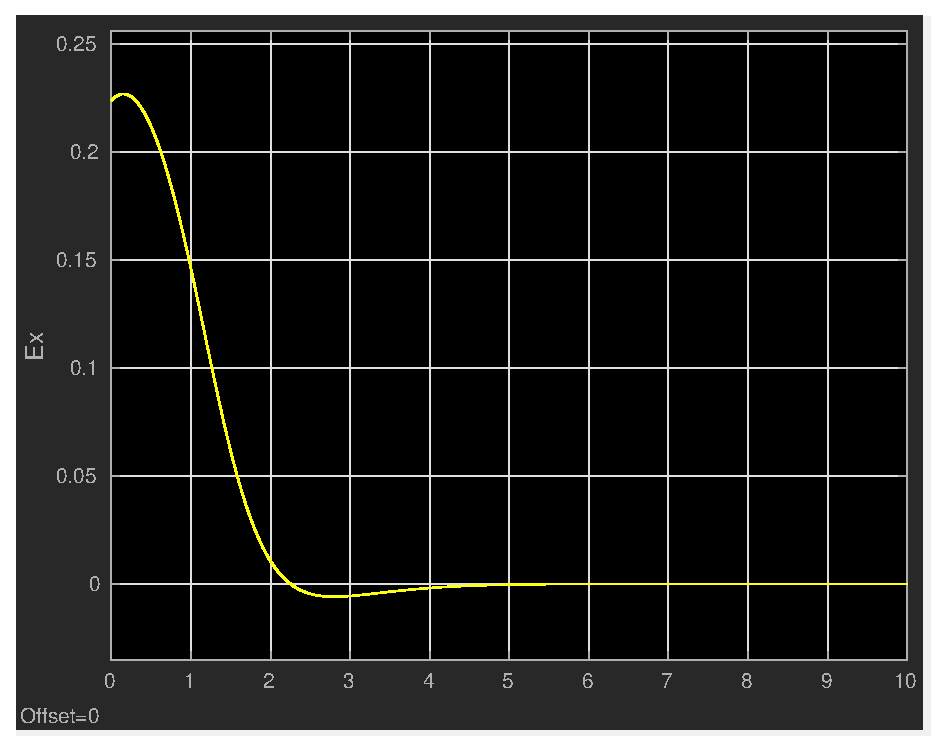
\includegraphics[width=0.5\textwidth]{images/simple_ex}}
	\caption{The horizontal error between the unit LOS vector and the unit optical axis vector converges to zero.}
	\label{simple_ex}
\end{figure}